En una carretera principal hi trobem el poble $A$. A 12 km del poble $A$, hi ha un encreuament $O$ amb una carretera
secundària que talla perpendicularment la carretera principal. A 9 km de l'encreuament, a la carretera secundària,
hi trobem el poble $B$. Es vol construir una torre de comunicacions $T$ en un punt de la carretera principal situat
entre el poble $A$ i l'encreuament $O$. Aquesta torre ha d'estar connectada amb cadascun dels dos pobles en línia recta
per cable. Sabem que instal·lar el cable entre la torre $T$ i el poble $B$ té un preu de 250 €/km i, en canvi,
instal·lar el cable entre la torre $T$ i el poble $A$ té un preu de 125 €/km.
\begin{center}
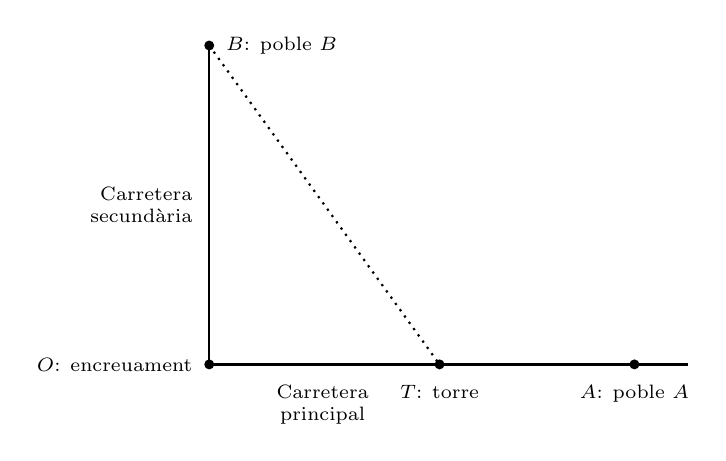
\begin{tikzpicture}[scale=0.45]
  \draw[thick] (0,9) -- (0,0) -- (13.5,0);
  \draw[dotted,thick] (0,9) -- (6.5,0);
  \fill (0,9) circle (4pt); \fill (0,0) circle (4pt); \fill (6.5,0) circle (4pt); \fill (12,0) circle (4pt);
  \node[right,font=\scriptsize] at (0.2,9) {$B$: poble $B$};
  \node[left,font=\scriptsize,align=right] at (-0.2,4.5) {Carretera\\secundària};
  \node[left,font=\scriptsize] at (-0.2,0) {$O$: encreuament};
  \node[below,font=\scriptsize,align=center] at (3.2,-0.3) {Carretera\\principal};
  \node[below,font=\scriptsize] at (6.5,-0.3) {$T$: torre};
  \node[below,font=\scriptsize] at (12,-0.3) {$A$: poble $A$};
\end{tikzpicture}
\end{center}

\begin{apartats}

\apartat{2,5}
Determineu a quina distància de l'encreuament $O$ a la carretera principal cal situar la torre $T$ perquè el preu del
cablejat sigui mínim, i quin serà el valor d'aquest preu mínim.

\begin{solucio}
Si denotem per $x$ la distància de l'encreuament a la torre, és a dir, $x=d(O,M)$, on $M$ és el punt on se situa la
torre, aleshores obtenim:
\begin{center}
\begin{tikzpicture}[scale=0.4]
  \draw (0,9) -- (0,0) -- (12,0);
  \draw[dashed] (0,9) -- (5.2,0);
  \fill (0,9) circle (3pt) node[above left,font=\scriptsize] {$B$};
  \fill (0,0) circle (3pt) node[below left,font=\scriptsize] {$O$};
  \fill (5.2,0) circle (3pt) node[below,font=\scriptsize] {$M$};
  \fill (12,0) circle (3pt) node[below,font=\scriptsize] {$A$};
  \node[left,font=\scriptsize] at (0,4.5) {$9$};
  \node[above,font=\scriptsize] at (2.6,0) {$x$};
  \node[above,font=\scriptsize] at (8.6,0) {$12-x$};
\end{tikzpicture}
\end{center}
Pel teorema de Pitàgores, veiem que $d(B,M)=\sqrt{81+x^2}$. Així doncs, el preu del cablejat vindrà donat per la
funció
\[
P(x)=125\,(12-x)+250\sqrt{81+x^2}.
\]
Per trobar el preu mínim, derivem la funció $P$:
\[
P'(x)=-125+250\cdot\frac{2x}{2\sqrt{81+x^2}}.
\]
Resolent $P'(x)=0$, obtenim $\sqrt{81+x^2}=2x$ i, elevant els dos membres al quadrat, tenim $81+x^2=4x^2$, que té com a
solució real positiva $x=\sqrt{27}=3\sqrt3$ km. Per comprovar que és un mínim, estudiem el signe de la derivada als
intervals $\left(0,3\sqrt3\right)$ i $\left(3\sqrt3,12\right)$: en el primer, $P'(x)<0$, i en el segon, $P'(x)>0$; per
tant, deduïm que el mínim de la funció $P$ s'assoleix per a $x=3\sqrt3$ km, és a dir, situant la torre a
$3\sqrt3\ \text{km}=5{,}2$ km de l'encreuament.

\textit{Pauta oficial:} 0,5 pel plantejament del problema, 0,5 per determinar la funció cost que cal optimitzar,
0,5 pel càlcul de la derivada primera, 0,5 per determinar el candidat a mínim, 0,25 per justificar que,
efectivament, correspon a un mínim, i 0,25 pel valor del cost mínim.

\textit{Nota del banc:} el criteri oficial no calcula el preu mínim, que l'enunciat demana i que la pauta puntua:
\[
P\!\left(3\sqrt3\right)=125\left(12-3\sqrt3\right)+250\sqrt{108}=1500-375\sqrt3+1500\sqrt3=1500+1125\sqrt3\approx3\,448{,}56\ \text{€}.
\]
És un mínim absolut a l'interval, perquè als extrems el preu és més alt: $P(0)=P(12)=3\,750$ €.
\end{solucio}

\end{apartats}
